
\title{A Taxonomy of Treemap Visualization Techniques}
\subtitle{IVAPP 2020}
\author{\underline{Willy Scheibel}, Matthias Trapp, Daniel Limberger, and Jürgen Döllner}
\institute{Hasso Plattner Institute, Digital Engineering Faculty, University of Potsdam}
\newcommand{\presentationdate}{\formatdate{29}{2}{2020}}
\date{\presentationdate}

\titlegraphic{
	\footnotesize
	\centering%
	\newlength{\definitionswidth}%
	\newlength{\definitionsheight}%
	\newlength{\definitionsoffset}%
	\newlength{\definitionsimagesize}%
	\newlength{\definitionsdescriptionsize}%
	\setlength{\definitionswidth}{\textwidth}%
	\setlength{\definitionsheight}{145pt}%
	\setlength{\definitionsoffset}{10pt}%
	\setlength{\definitionsimagesize}{0.25\definitionswidth - 2\definitionsoffset}%
	\setlength{\definitionsdescriptionsize}{0.25\definitionswidth - 0.5\definitionsoffset}%
	\begin{tikzpicture}[]
	\node[inner sep=0,outer sep=0] (space-filling) at (-1.5\definitionsimagesize - 3\definitionsoffset, 0.5\definitionsheight) {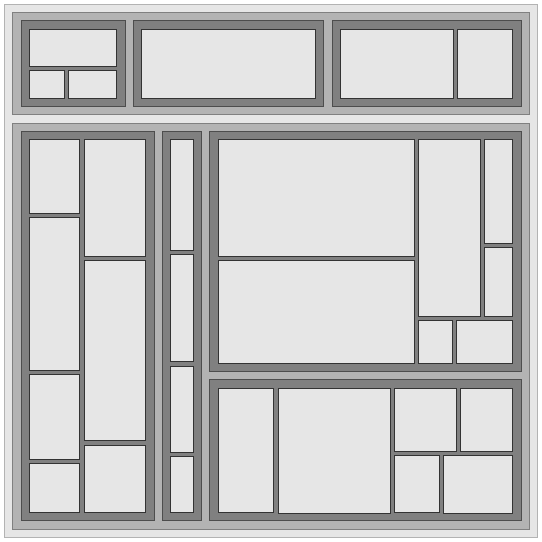
\includegraphics[width=\definitionsimagesize]{figures/treemap-cat-s}};
	\node[inner sep=0,outer sep=0] (containment) at (-0.5\definitionsimagesize + -1\definitionsoffset, 0.5\definitionsheight) {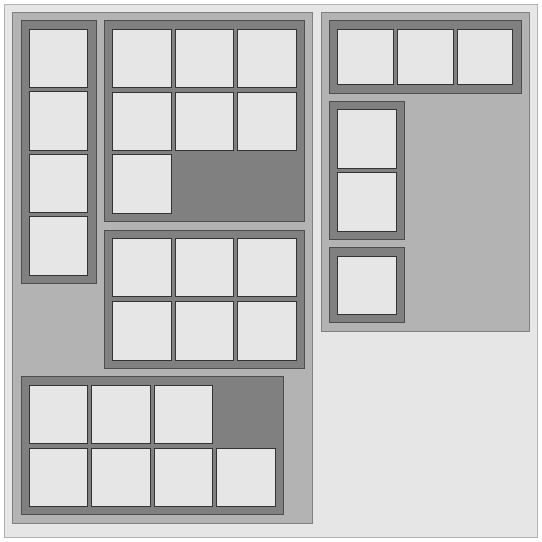
\includegraphics[width=\definitionsimagesize]{figures/treemap-cat-c}};
	\node[inner sep=0,outer sep=0] (implicit-edge) at (0.5\definitionsimagesize + 1\definitionsoffset, 0.5\definitionsheight) {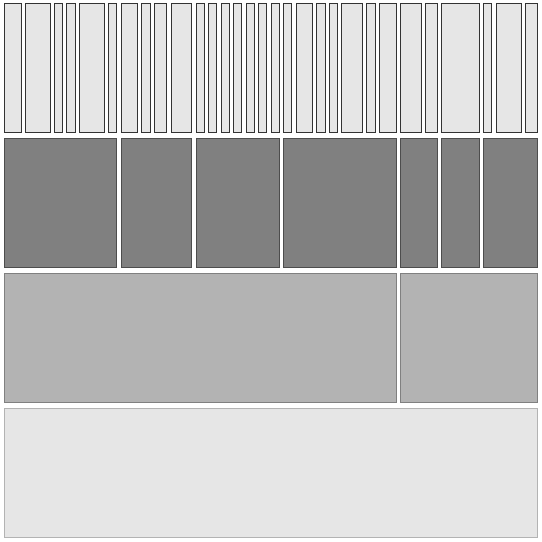
\includegraphics[width=\definitionsimagesize]{figures/treemap-cat-ie}};
	\node[inner sep=0,outer sep=0] (mapped-tree) at (1.5\definitionsimagesize + 3\definitionsoffset, 0.5\definitionsheight) {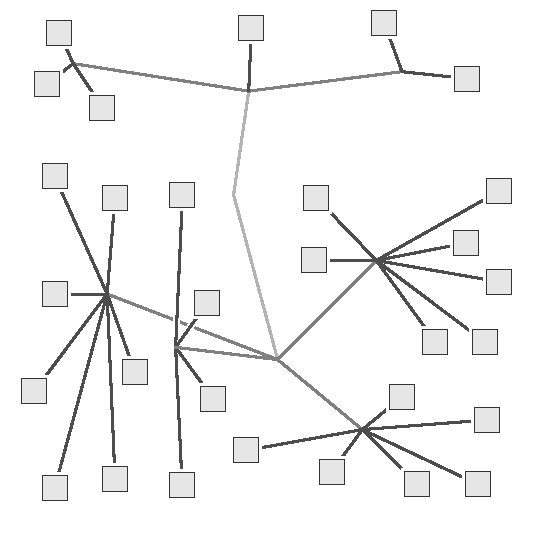
\includegraphics[width=\definitionsimagesize]{figures/treemap-cat-mt}};
	\node[draw=none] (annotation-center) at (0, 0.15\definitionsheight) {};
	\node[above=0cm of space-filling] (tm0) {\Ts};
	\node[below=0cm of space-filling,text width=\definitionsdescriptionsize,align=center] (tm0-description) { Space-filling Treemap };
	\node[above=0cm of containment] (tm1) {\Tc};
	\node[below=0cm of containment,text width=\definitionsdescriptionsize,align=center] (tm1-description) { Containment Treemap };
	\node[above=0cm of implicit-edge] (tm2) {\Tie};
	\node[below=0cm of implicit-edge,text width=\definitionsdescriptionsize,align=center] (tm2-description) { Implicit Edge Representation Tree };
	\node[above=0cm of mapped-tree] (tm3) {\Tmt};
	\node[below=0cm of mapped-tree,text width=\definitionsdescriptionsize,align=center] (tm3-description) { Mapped Tree };
	\end{tikzpicture}%
}
